\documentclass[11pt,en]{elegantpaper}
\title{Quantitative Risk Management Project 5}
\author{Qijun Yang \\ Duke University}
\institute{\href{https://fintech.meng.duke.edu}{Financial Technology at Duke University}}
\version{1.0}
\date{Feb. 25, 2023}

% cmd for this doc
\usepackage{array}
\usepackage{listings}
\usepackage{graphicx}
\usepackage{subfigure}
\newcommand{\ccr}[1]{\makecell{{\color{#1}\rule{1cm}{1cm}}}}

\addbibresource[location=local]{reference.bib} % reference file
\begin{document}
\maketitle

\section*{\textcolor{orange}{Problem 1}}

Use the data in problem1.csv. Fit a Normal Distribution and a Generalized T distribution to this data.
Calculate the VaR and ES for both fitted distributions.

Overlay the graphs the distribution PDFs, VaR, and ES values. What do you notice? Explain the
differences.

\section*{\textcolor{orange}{Answer}}

\subsection*{\textcolor{orange}{1. Finding:}}


We use data to construct MLE fitted Normal and T distribution then we calculate the corresponding VaR and Expected Shortfall.
\begin{enumerate}
 \item For both fitted normal and T, their Expected Shortfall is larger than VaR, which can also be proved by math. See the following.
 \item We could find that the VaR of the fitted normal distribution is larger than that of the fitted T distribution but the Expected Shortfall of the fitted T distribution is larger than that of fitted normal distribution. 
\end{enumerate}

\subsection*{\textcolor{orange}{2. Reasoning:}}

The reason why this w will happen is that the fitted T distribution has a heavier tail than the fitted normal. Expected Shortfall is the average of the VaRs which are larger than the VaR at tail probability alpha when the underlying distribution is continuous. 

VaR only measures the maximum loss given a certain confidence interval, ignoring the possibility of extreme losses outside of that threshold. 
That means VaR ignores the tail risk.

Expected Shortfall could tackle such a problem. It considers the whole tail risk and averages them to get an expected potential loss. Even though at some times, the Var is low but the Expected Shortfall may be very high.

Therefore, we could not only use VaR to help us discover the risk level of our portfolio. We should combine VaR and ES to have a better understanding.

\begin{table}[htbp]
    \centering
    \caption{Time period = 1}
    \begin{tabular}{@{}ccccc@{}}
        \toprule
        \textbf{Risk Metrics} & \textbf{Distribution} & \textbf{Value}\\
        \midrule
        VaR & Normal  & 0.08125  \\
        & T  & 0.07648     \\
        Expected Shortfall & Normal  & 0.1017 \\
        & T & 0.1132 \\
        \bottomrule
    \end{tabular}
\end{table}

\begin{figure}[htbp] 
    \centering 
    \includegraphics[width=0.8\textwidth]{./image/ES_VaR.png} 
\end{figure}

\subsection*{\textcolor{orange}{3. Mathematical Reasoning:}}

The finding that Expected Shortfall is bigger than VaR can be proved:

If we assume the distribution is continuous, then we have 
\[
    \begin{aligned}
    ES_{\alpha}(X)&=-\frac{1}{\alpha}\int_{0}^{\alpha}VaR_p(X)dp\\
    &=E(-X|X\leq-VaR_\alpha(X))\\
    &=E(-X-VaR_\alpha(X)+VaR_\alpha(X)|X\leq-VaR_\alpha(X))\\
    &=E(-X-VaR_\alpha(X)|X\leq-VaR_\alpha(X))+E(VaR_\alpha(X)|X\leq-VaR_\alpha(X))\\
    &=VaR_\alpha(X)-E((X+VaR_\alpha(X))^{-}|X\leq-VaR_\alpha(X))\\
    &\geq VaR_\alpha(X)
    \end{aligned}
\]


\section*{\textcolor{orange}{Problem 2}}
    In your main repository, create a Library for risk management. Create modules, classes, packages, etc
    as you see fit. Include all the functionality we have discussed so far in class. 
    
    Make sure it includes
    \begin{enumerate}
        \item Covariance estimation techniques.
        \item Non PSD fixes for correlation matrices
        \item Simulation Methods
        \item VaR calculation methods (all discussed)
        \item ES calculation
    \end{enumerate}

    Create a test suite and show that each function performs as expected.
    


\section*{\textcolor{orange}{Answer}}
    
    All the test is passed. Please refer to my Github.

    \begin{figure}[htbp] 
        \centering 
        \includegraphics[width=0.6\textwidth]{./image/test.png} 
    \end{figure}

\section*{\textcolor{orange}{Problem 3}}
    Use your repository from \#2.

    Using Portfolio.csv and DailyPrices.csv. Assume the expected return on all stocks is 0.

    This file contains the stock holdings of 3 portfolios. You own each of these portfolios.

    Fit a Generalized T model to each stock and calculate the VaR and ES of each portfolio as well as your
    total VaR and ES. 
    
    Compare the results from this to your VaR form Problem 3 from Week 4.

\section*{\textcolor{orange}{Answer}}

Assume the return of all stocks follow generalized T distribution, we use the return data to construct the Gaussian Copula and use Gaussian Copula to simulate the T distributed return.

Gaussian Copula:
\[C_R^{Gauss}(u)=\Phi_R(\Phi^{-1}(u_1),\cdots,\Phi^{-1}(u_n))\]
where $\Phi^{-1}$ is the inverse cumulative distribution function of a standard normal and $\Phi_R$ is the joint cumulative distribution function of a multivariate normal distribution with mean vector zero and covariance matrix equal to the correlation matrix $R$.

\subsection*{\textcolor{orange}{Finding:}}

We find the Generalized T model will result in larger VaR and ES than other methods of Normal, like Normal-Delta and Normal Monte Carlo Simulation. 

\begin{table}[htbp]
    \centering
    \caption{VaR of Portfolio}
    \begin{tabular}{@{}cccccc@{}}
        \toprule
        \textbf{Risk Metrics} & \textbf{Method} &\textbf{portfolio A} & \textbf{portfolio B} & \textbf{portfolio C} & \textbf{Total portfolio}\\
        \midrule
        VaR & Normal-Delta & 5678.98  & 4492.44 & 3775.87 & 13570.22 \\
        & Normal MC & 5670.20  & 4494.59 & 3786.58 & 13577.07 \\
        & Historical Simulation & 9070.10  & 7351.16 & 5802.652 & 21275.01 \\
        & T + Gaussian Copula & 7866.03  & 6908.44 & 5742.72 & 20288.10 \\
        ES & Normal MC & 7155.39  & 5635.36 & 4759.14 & 7031.40 \\
        & Historical Simulation & 10640.56  & 9183.29 & 7568.59 & 26579.18 \\
        & T + Gaussian Copula & 10573.47  & 9221.20 & 7755.23 & 26418.80 \\
        \bottomrule
    \end{tabular}
\end{table}
 
As we can see from the chart that for VaR, under Normal assumption, the portfolio has the samllest Value at Risk. Under the T assumption, the portfolio has almost same VaR as Historical Simulation except fot portfolio C. 

Therefore, we can tell that Generalized T model could better catch the Value at Risk even though there is some difference between Historical Simulation and Generalized T model. For the Normal Model, it underestimate the potential loss.

As to Expected Shortfall, the order of three Model is very clear. THe ES of Generalized T model is the largest and the ES of Normal is the samllest. The Historical ES is in the middel of those two.


We could also see there are more outliers in the Generalized T model. It's not surprise this will happen. The T Model capture more information of the tail. It considers more tail risk than normal.

\newpage
\begin{figure}[htbp]
    \centering
    \subfigure[Portfolio A]{
    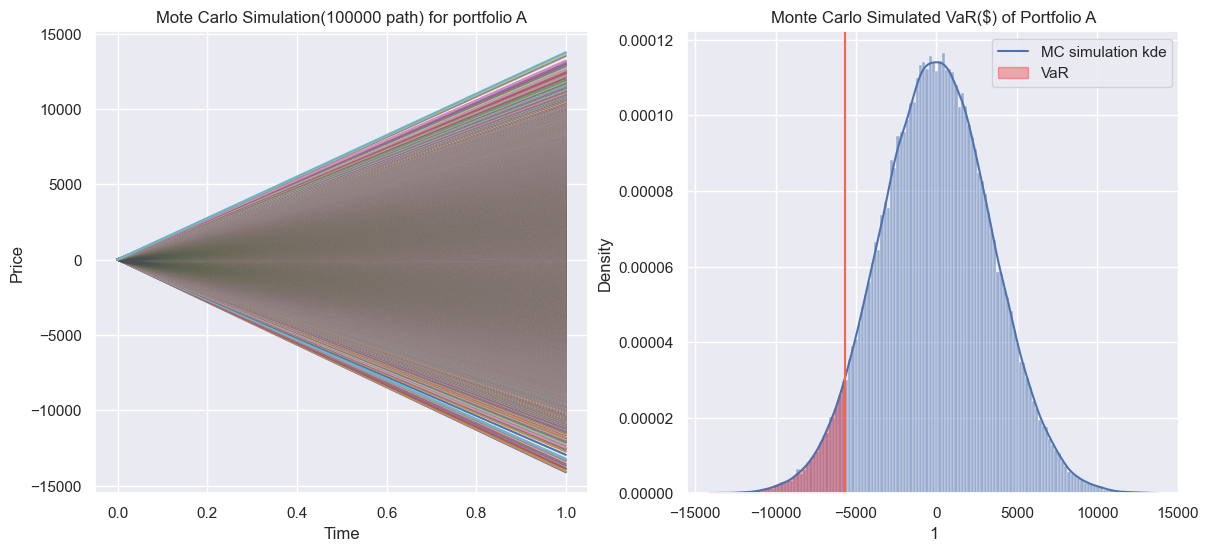
\includegraphics[width=0.58\textwidth]{./image/MC_A.png} 
    }
    \quad
    \subfigure[Portfolio B]{
    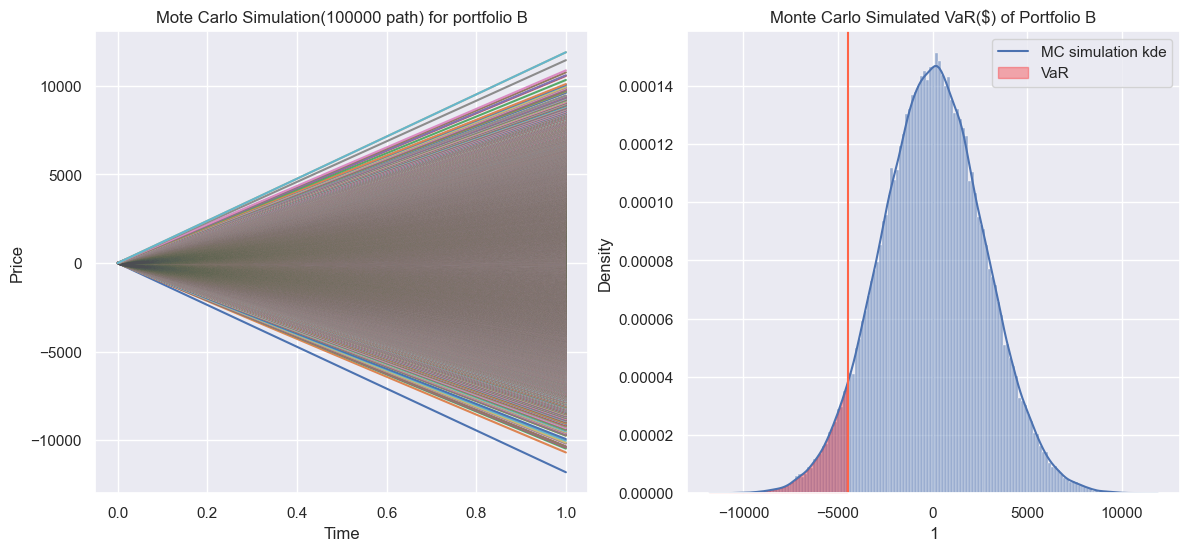
\includegraphics[width=0.58\textwidth]{./image/MC_B.png} 
    }
    \quad
    \subfigure[Portfolio C]{
    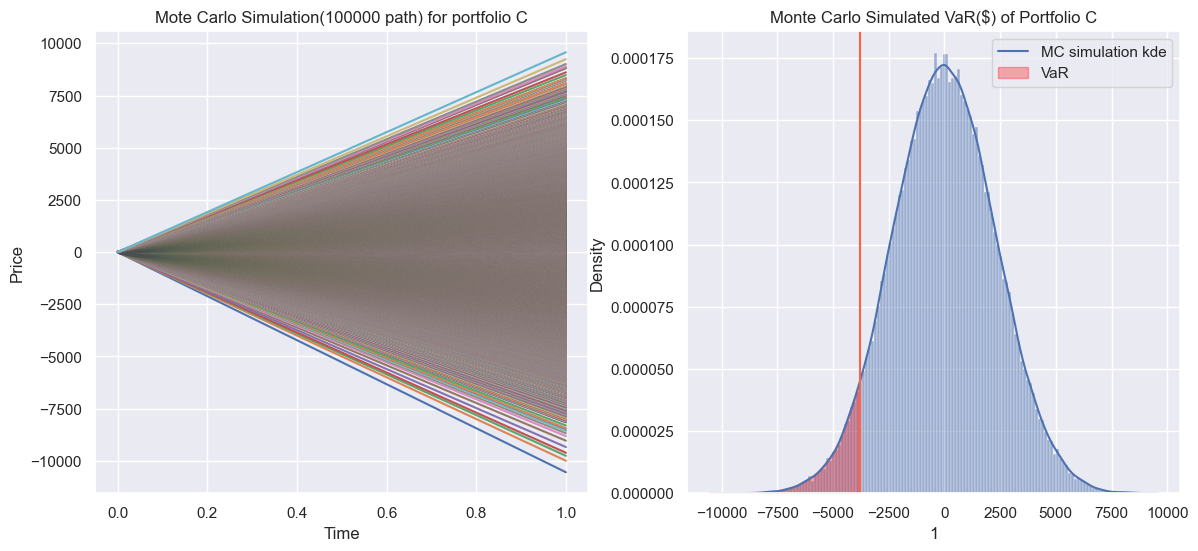
\includegraphics[width=0.58\textwidth]{./image/MC_C.png} 
    }
    \quad
    \subfigure[Portfolio ALL]{
    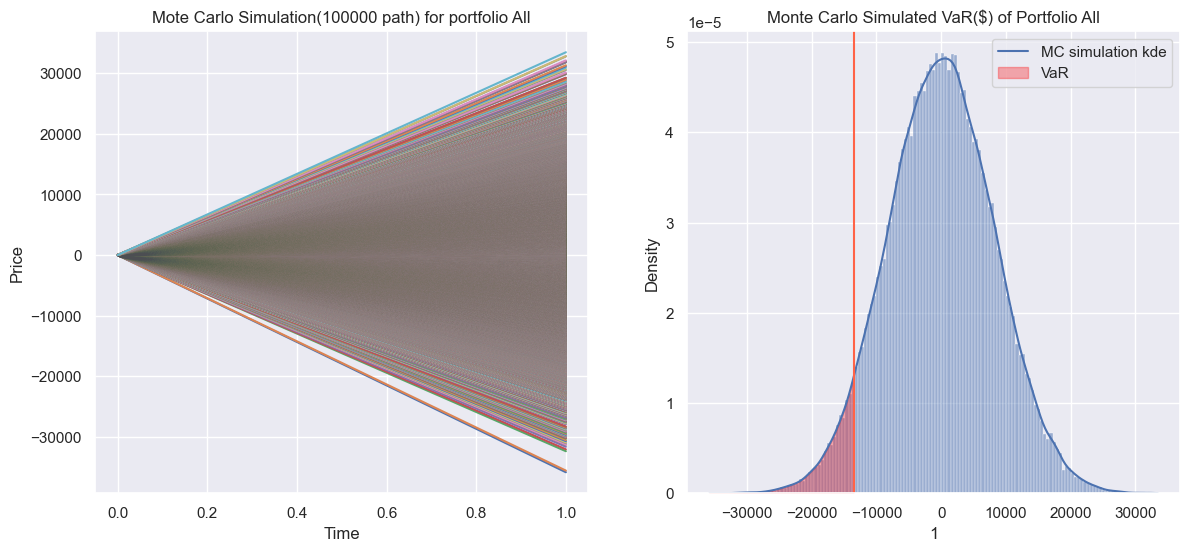
\includegraphics[width=0.58\textwidth]{./image/MC_ALL.png} 
    }
    \caption{Normal Model Carlo Simulation}
\end{figure}

\newpage
\begin{figure}[htbp]
    \centering
    \subfigure[Portfolio A]{
    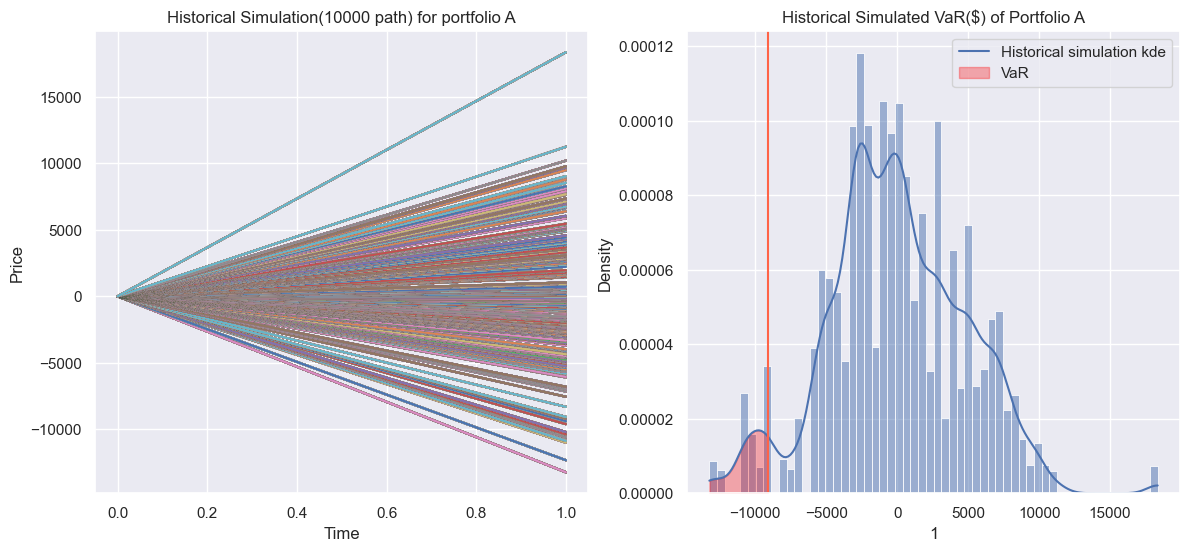
\includegraphics[width=0.58\textwidth]{./image/His_A.png} 
    }
    \quad
    \subfigure[Portfolio B]{
    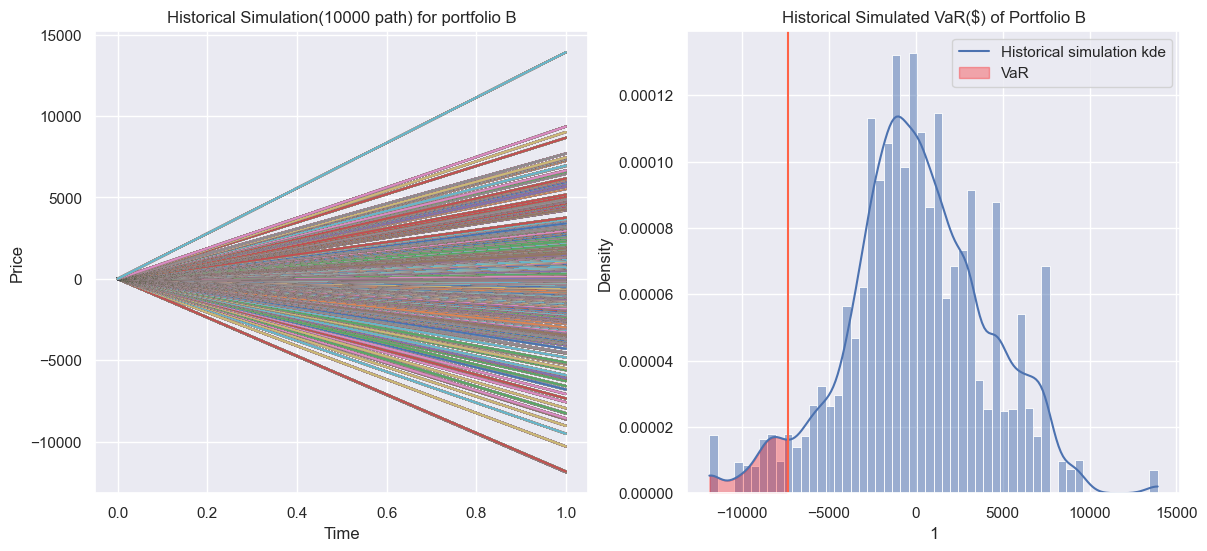
\includegraphics[width=0.58\textwidth]{./image/His_B.png} 
    }
    \quad
    \subfigure[Portfolio C]{
    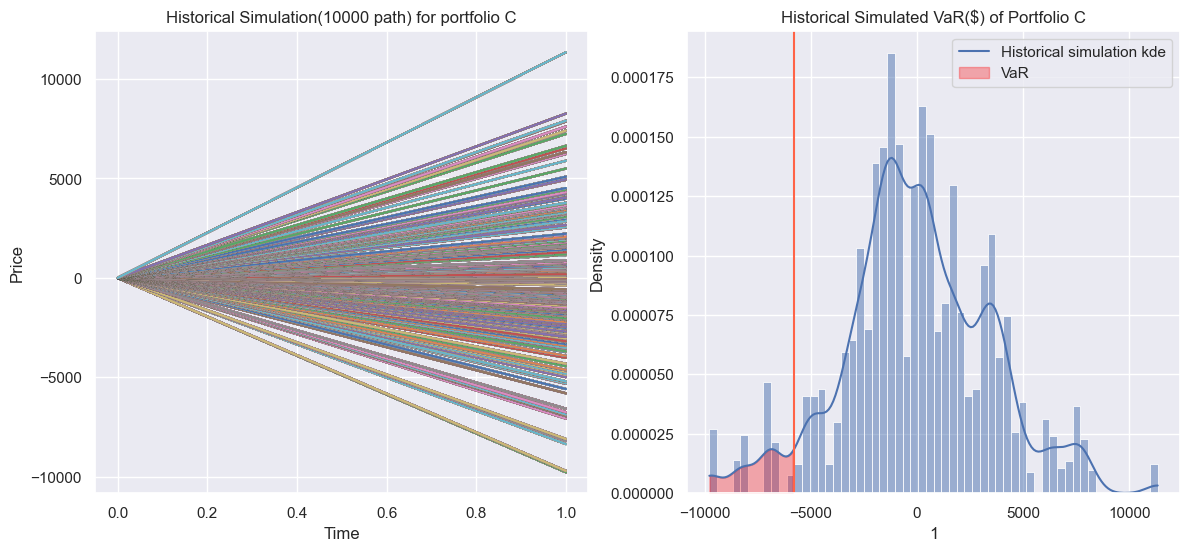
\includegraphics[width=0.58\textwidth]{./image/His_C.png} 
    }
    \quad
    \subfigure[Portfolio ALL]{
    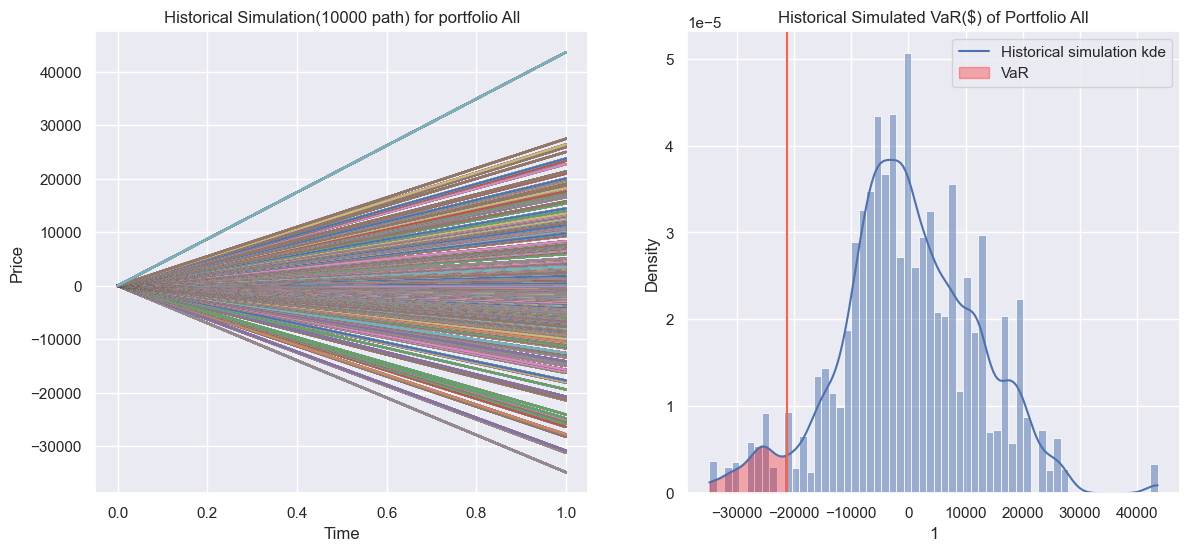
\includegraphics[width=0.58\textwidth]{./image/His_ALL.png} 
    }
    \caption{Historical Simulation}
\end{figure}

\newpage

\begin{figure}[htbp]
    \centering
    \subfigure[Portfolio A]{
    \includegraphics[width=0.58\textwidth]{./image/T_A.png} 
    }
    \quad
    \subfigure[Portfolio B]{
    \includegraphics[width=0.58\textwidth]{./image/T_B.png} 
    }
    \quad
    \subfigure[Portfolio C]{
    \includegraphics[width=0.58\textwidth]{./image/T_C.png} 
    }
    \quad
    \subfigure[Portfolio ALL]{
    \includegraphics[width=0.58\textwidth]{./image/T_ALL.png} 
    }
    \caption{Generalized T model}
\end{figure}

\end{document}